\documentclass[multi=tikzpicture,border=7pt]{standalone}
\usepackage{ctex,amsmath,amssymb,bm}
\usepackage{tikz,pgfplots}
\pgfplotsset{compat=1.18}
\usetikzlibrary{arrows.meta,calc,angles,quotes,patterns,positioning,decorations.pathmorphing,3d,intersections}
\tikzset{wire/.style={brown!70!black,very thick},guide/.style={dashed,gray!60},force/.style={->,>=Stealth,thick,red!70!black},velocity/.style={->,>=Stealth,thick,blue!70!black},axis/.style={->,>=Stealth,thick},dim/.style={<->,>=Stealth,thin},body/.style={draw,thick,fill=blue!7},panel/.style={anchor=west,font=\bfseries},hidden/.style={dashed,gray!58,thick},orbit/.style={very thick,blue!70!black}}
\tikzset{charge/.style={circle,draw,fill=blue!12,minimum size=5.5mm,inner sep=0pt},resistor/.style={decorate,decoration={zigzag,segment length=4pt,amplitude=2pt},thick}}
\tikzset{vec/.style={->,>=Stealth,very thick},wall/.style={pattern=north east lines,pattern color=gray},nodept/.style={circle,fill=white,draw,inner sep=1.5pt}}
\tikzset{flow/.style={->,>=Stealth,very thick,blue!70!black},current/.style={->,>=Stealth,very thick,red!70!black},terminal/.style={circle,draw,fill=white,inner sep=1.5pt}}
\begin{document}
% 1 question-01
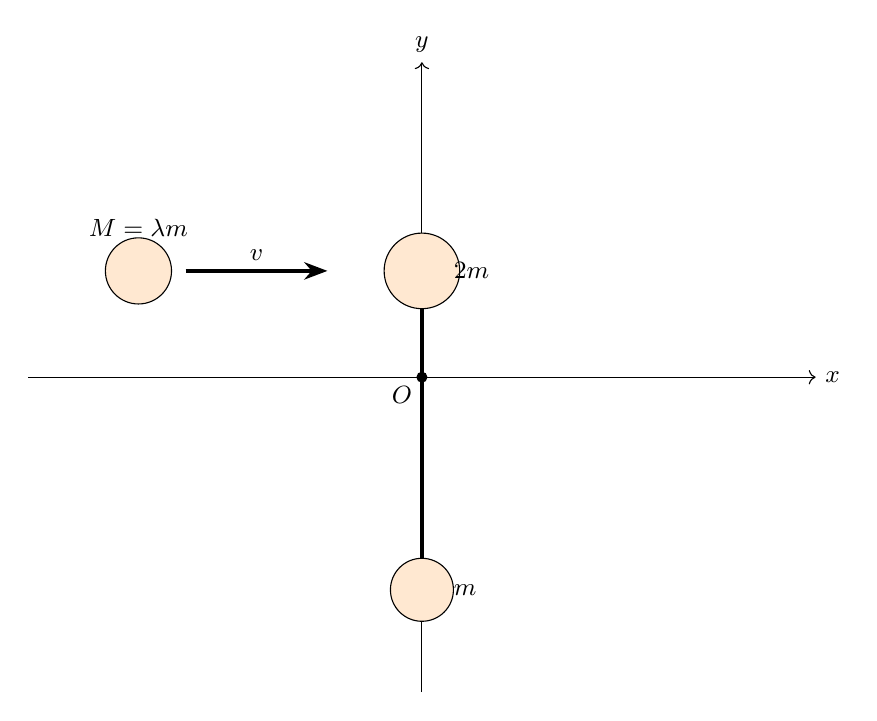
\begin{tikzpicture}[x=1cm,y=1cm,font=\small]

\draw[->] (-5,0)--(5,0) node[right] {$x$}; \draw[->] (0,-4)--(0,4) node[above] {$y$};
 \draw[very thick] (0,-2.7)--(0,1.35);
 \draw[draw=black,fill=orange!18] (0,1.35) circle (.48) node[right=8pt] {$2m$};
 \draw[draw=black,fill=orange!18] (0,-2.7) circle (.4) node[right=8pt] {$m$};
 \draw[draw=black,fill=orange!18] (-3.6,1.35) circle (.42) node[above=9pt] {$M=\lambda m$};
 \draw[vec,very thick] (-3,1.35)--(-1.2,1.35) node[midway,above] {$v$};
 \fill (0,0) circle (2pt) node[below left] {$O$};

\end{tikzpicture}

% 2 solution-01
\begin{tikzpicture}[x=1cm,y=1cm,font=\small]

\draw[->] (-5.5,0)--(4.5,0) node[right] {$x$};
 \draw[guide] (-5,1)--(4,1) node[right] {$y=l/3$};
 \fill (0,0) circle (2pt) node[below right] {$O$};
 \draw[guide,thick] (0,-2)--(0,1);
 \draw[draw=black,fill=orange!18] (0,1) circle (.30);
 \draw[draw=black,fill=orange!18] (0,-2) circle (.27);
 \node[gray!78] at (.7,-1.8) {初始位置};
 \draw[very thick,blue!70!black] (-1.732,1)--(.866,-.5);
 \draw[draw=black,fill=orange!18] (-1.732,1) circle (.32) node[above] {$m$};
 \draw[draw=black,fill=orange!18] (.866,-.5) circle (.36) node[right] {$2m$};
 \draw[vec,blue!70!black] (0,1.45) arc (90:-30:1.45);
 \node[blue!70!black] at (1.55,.72) {$\phi_*=2\pi/3$};
 \draw[draw=black,fill=orange!18] (-.82,1) circle (.34) node[above=4pt] {$M$};
 \draw[vec,red!70!black] (-.95,1)--(-2.6,1) node[midway,above] {$u$};
 \draw[<->] (0,-2.8)--(-1.732,-2.8) node[midway,below] {$\sqrt3\,l/3$};
 \draw[guide] (-1.732,1)--(-1.732,-3.05);
 \node[align=left] at (4,-2) {$t_*=\dfrac{2\pi}{3\omega}$\\[5pt]
 $s_M=ut_*$\\[4pt]临界条件：$s_M\le \dfrac{\sqrt3 l}{3}$};

\end{tikzpicture}

% 3 question-02
\begin{tikzpicture}[x=1cm,y=1cm,font=\small]

\fill[gray!15] (-5,-.28) rectangle (5,0); \draw[very thick] (-5,0)--(5,0);
 \draw[guide] (0,-3.4)--(0,4.1);
 \fill (0,2.4) circle (2pt) node[below right] {$O$};
 \draw[very thick] (-1.27,1.81)--(1.27,2.99);
 \draw[draw=black,fill=orange!18] (-1.27,1.81) circle (.35) node[left=4pt] {$m_1,-q_1$};
 \draw[draw=black,fill=orange!18] (1.27,2.99) circle (.35) node[right=4pt] {$m_2,q_2$};
 \draw[guide] (0,2.4)--(0,4);
 \draw[blue!70!black,->] (0,3.35) arc (90:25:0.95);
 \node[blue!70!black] at (.58,3.52) {$\theta$};
 \draw[<->] (-2.35,0)--(-2.35,2.4) node[midway,left] {$h$};
 \node at (3.9,.42) {接地导体板};

\end{tikzpicture}

% 4 solution-02
\begin{tikzpicture}[x=1cm,y=1cm,font=\small]

\begin{scope}[shift={(-3.3,0)}]
\draw[thick](-2.3,0)--(2.3,0);\node at(0,-2.4){接地面及镜像（非同比例）};
\draw[thick](-.8,1.4)--(.8,2.4);\fill(0,1.9)circle(2pt)node[left]{$O$};
\foreach\x/\y/\a/\b in{-.8/1.4/{-q_1}/{+q_1},.8/2.4/{q_2}/{-q_2}}{
\draw[charge](\x,\y)circle(.13)node[above]{$\a$};\draw[charge](\x,-\y)circle(.13)node[below]{$\b$};\draw[guide](\x,\y)--(\x,-\y);}
\draw[dim](-2,0)--(-2,1.9)node[midway,left]{$h$};
\end{scope}
\begin{scope}[shift={(.1,-1.5)}]
\draw[axis](0,0)--(5,0)node[right]{$\theta$};\draw[axis](0,-.5)--(0,3)node[above]{$(U-U_0)/K$};
\draw[orbit,domain=0:180,samples=151]plot({\x/40},{2+cos(\x)-cos(\x)^2});
\foreach\t/\y/\lab in{0/2/{0},60/2.25/{\pi/3},180/0/{\pi}}{\fill(\t/40,\y)circle(2pt);\draw[guide](\t/40,0)--(\t/40,\y);\node[below]at(\t/40,0){$\lab$};}
\node[above right]at(0,2){稳定};\node[above]at(1.5,2.25){不稳定};\node[above left]at(4.5,0){稳定};
\node[align=center]at(2.5,-1){$K=\tfrac25mgh\,a^2$；曲线整体上移2\\仅为 $a\ll1$ 的二阶近似};
\end{scope}

\end{tikzpicture}

% 5 question-03
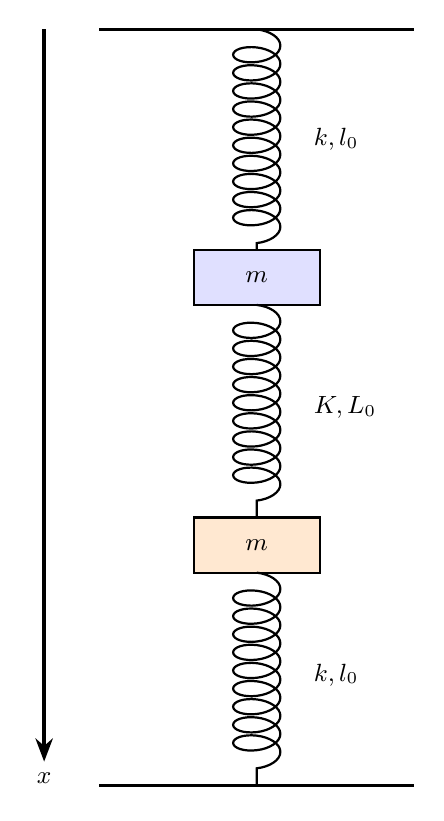
\begin{tikzpicture}[x=1cm,y=1cm,font=\small]

\draw[very thick] (-2,4.8)--(2,4.8) (-2,-4.8)--(2,-4.8);
 \draw[decorate,decoration={coil,segment length=2.3mm,amplitude=3mm},thick] (0,4.8)--(0,2);
 \draw[fill=blue!12,thick] (-.8,1.3) rectangle (.8,2) node[midway] {$m$};
 \draw[decorate,decoration={coil,segment length=2.3mm,amplitude=3mm},thick] (0,1.3)--(0,-1.4);
 \draw[fill=orange!18,thick] (-.8,-2.1) rectangle (.8,-1.4) node[midway] {$m$};
 \draw[decorate,decoration={coil,segment length=2.3mm,amplitude=3mm},thick] (0,-2.1)--(0,-4.8);
 \node[right] at (.6,3.4) {$k,l_0$}; \node[right] at (.6,0) {$K,L_0$}; \node[right] at (.6,-3.4) {$k,l_0$};
 \draw[vec] (-2.7,4.8)--(-2.7,-4.5) node[below] {$x$};

\end{tikzpicture}

% 6 solution-03
\begin{tikzpicture}[x=1cm,y=1cm,font=\small]

\begin{scope}[shift={(-4,0)}]
  \draw[very thick] (-1,3)--(1,3) (-1,-3)--(1,-3);
  \draw[decorate,decoration={coil,segment length=2mm,amplitude=2mm}] (0,3)--(0,1);
  \filldraw[fill=blue!15] (-.5,.6) rectangle (.5,1);
  \draw[decorate,decoration={coil,segment length=2mm,amplitude=2mm}] (0,.6)--(0,-.6);
  \filldraw[fill=blue!15] (-.5,-1) rectangle (.5,-.6);
  \draw[decorate,decoration={coil,segment length=2mm,amplitude=2mm}] (0,-1)--(0,-3);
  \draw[force] (.8,.8)--(.8,-.2); \draw[force] (.8,-.8)--(.8,-1.8);
  \node at (0,3.7) {同相};
 \end{scope}
 \begin{scope}[shift={(3,0)}]
  \draw[very thick] (-1,3)--(1,3) (-1,-3)--(1,-3);
  \draw[decorate,decoration={coil,segment length=2mm,amplitude=2mm}] (0,3)--(0,1);
  \filldraw[fill=orange!18] (-.5,.6) rectangle (.5,1);
  \draw[decorate,decoration={coil,segment length=1.6mm,amplitude=3mm}] (0,.6)--(0,-.6);
  \filldraw[fill=orange!18] (-.5,-1) rectangle (.5,-.6);
  \draw[decorate,decoration={coil,segment length=2mm,amplitude=2mm}] (0,-1)--(0,-3);
  \draw[force] (.8,.8)--(.8,-.2); \draw[force] (.8,-.8)--(.8,.2);
  \node at (0,3.7) {反相};
 \end{scope}
 \node[align=left] at (8,1.2) {$\omega_1=\sqrt{k/m}$\\[7pt]$\omega_2=\sqrt{(k+2K)/m}$\\[7pt]
 $x_a=(q_1+q_2)/2$\\ $x_b=(q_1-q_2)/2$};

\end{tikzpicture}

% 7 question-04
\begin{tikzpicture}[x=1cm,y=1cm,font=\small]

\draw (0,0)--(0,4)--(2,4);
 \draw[decorate,decoration={coil,segment length=3mm,amplitude=3mm},thick] (2,4)--(4,4) node[midway,above=6pt] {$L$};
 \draw[thick] (4,3.5)--(4,4.5) (4.45,3.65)--(4.45,4.35); \node at (4.25,4.9) {$C$};
 \draw (4.45,4)--(8,4)--(8,0);
 \draw[thick] (0,1.7) rectangle (1.7,2.3) node[midway] {$R$};
 \draw (1.7,2)--(5.3,2); \draw[thick,fill=orange!20] (5.3,1.6) rectangle (7,2.4) node[midway] {$-r$};
 \draw (7,2)--(8,2);
 \draw[vec,red!70!black] (3.8,3.5)--(1.6,3.5) node[midway,above] {$i(t)$};
 \draw (0,0)--(.6,0);
 \draw[decorate,decoration={coil,segment length=2.2mm,amplitude=2.5mm},thick] (.6,0)--(2.7,0);
 \draw (2.7,0)--(5.1,0);
 \draw[thick] (5.1,-.48)--(5.1,.48) (5.48,-.3)--(5.48,.3);
 \draw (5.48,0)--(8,0);
 \node[above] at (1.65,.35) {RFC};
 \node[below] at (5.3,-.45) {$V_b$};
 \draw[vec,blue!70!black] (3.8,-.38)--(2.5,-.38) node[midway,below] {$I$};
 \node at (4,-1.25) {直流偏置支路与交流谐振回路};

\end{tikzpicture}

% 8 solution-04
\begin{tikzpicture}[x=1cm,y=1cm,font=\small]

\draw[->] (0,0)--(7,0) node[right] {$t$}; \draw[->] (0,-4)--(0,4.5) node[above] {$i$};
 \draw[very thick,blue!70!black,domain=0:6.2,samples=150] plot (\x,{.35*exp(.22*\x)*sin(300*\x)});
 \draw[red!70!black,dashed,domain=0:6.2,samples=80] plot (\x,{.35*exp(.22*\x)});
 \draw[red!70!black,dashed,domain=0:6.2,samples=80] plot (\x,{-.35*exp(.22*\x)});
 \node[align=left] at (10,2.4) {$\ddot i+\dfrac{R-r}{L}\dot i+\dfrac{i}{LC}=0$\\[7pt]
 $R<r<R+2\sqrt{L/C}$\\[7pt]
 $\displaystyle f=\frac1{2\pi}\sqrt{\frac1{LC}-\frac{(R-r)^2}{4L^2}}$};


\end{tikzpicture}

% 9 question-05
\begin{tikzpicture}[x=1cm,y=1cm,font=\small]

\draw[thick] (0,0) circle (3.5); \fill (0,0) circle (2pt) node[below] {$O$};
 \draw[->] (0,0)--(4.5,0) node[right] {极轴};
 \draw[very thick,blue!70!black,domain=0:90,samples=100,variable=\t]
 plot ({(3.5*\t/90)*cos(\t)},{(3.5*\t/90)*sin(\t)});
 \draw[draw=black,fill=orange!18] (0,3.5) circle (.25) node[above] {小虫};
 \node at (-1.4,1.2) {$r=2R\theta/\pi$};

\end{tikzpicture}

% 10 solution-05
\begin{tikzpicture}[x=1cm,y=1cm,font=\small]

\draw[axis](-.2,0)--(3.2,0)node[right]{$4x/R$};\draw[axis](0,-.2)--(0,2.8)node[above]{$4y/R$};
\draw[orbit]plot coordinates{(0.00000,0.00000) (0.01258,0.00012) (0.02515,0.00050) (0.03772,0.00112) (0.05028,0.00199) (0.06282,0.00310) (0.07534,0.00447) (0.08784,0.00608) (0.10032,0.00794) (0.11276,0.01004) (0.12517,0.01239) (0.13755,0.01498) (0.14989,0.01782) (0.16218,0.02090) (0.17443,0.02422) (0.18662,0.02778) (0.19877,0.03157) (0.21085,0.03561) (0.22287,0.03988) (0.23484,0.04439) (0.24673,0.04913) (0.25855,0.05410) (0.27030,0.05930) (0.28197,0.06473) (0.29357,0.07039) (0.30508,0.07627) (0.31650,0.08237) (0.32784,0.08869) (0.33908,0.09524) (0.35023,0.10199) (0.36128,0.10897) (0.37224,0.11615) (0.38309,0.12354) (0.39383,0.13115) (0.40447,0.13895) (0.41500,0.14696) (0.42541,0.15517) (0.43572,0.16358) (0.44590,0.17218) (0.45597,0.18097) (0.46591,0.18996) (0.47573,0.19913) (0.48543,0.20848) (0.49499,0.21802) (0.50443,0.22774) (0.51374,0.23763) (0.52292,0.24769) (0.53196,0.25793) (0.54087,0.26833) (0.54964,0.27890) (0.55827,0.28964) (0.56676,0.30053) (0.57511,0.31157) (0.58332,0.32277) (0.59138,0.33413) (0.59930,0.34562) (0.60708,0.35727) (0.61470,0.36905) (0.62218,0.38098) (0.62951,0.39304) (0.63670,0.40523) (0.64373,0.41756) (0.65061,0.43001) (0.65734,0.44259) (0.66392,0.45529) (0.67035,0.46810) (0.67662,0.48104) (0.68274,0.49408) (0.68871,0.50724) (0.69453,0.52051) (0.70019,0.53388) (0.70570,0.54735) (0.71105,0.56092) (0.71625,0.57459) (0.72130,0.58835) (0.72619,0.60220) (0.73093,0.61614) (0.73551,0.63017) (0.73995,0.64428) (0.74423,0.65847) (0.74835,0.67274) (0.75233,0.68709) (0.75615,0.70151) (0.75982,0.71600) (0.76334,0.73056) (0.76671,0.74519) (0.76993,0.75988) (0.77300,0.77463) (0.77592,0.78944) (0.77870,0.80430) (0.78132,0.81922) (0.78380,0.83420) (0.78613,0.84922) (0.78832,0.86430) (0.79036,0.87942) (0.79226,0.89458) (0.79402,0.90978) (0.79563,0.92503) (0.79710,0.94031) (0.79843,0.95563) (0.79963,0.97099) (0.80068,0.98637) (0.80160,1.00179) (0.80237,1.01724) (0.80302,1.03271) (0.80353,1.04821) (0.80390,1.06373) (0.80414,1.07927) (0.80426,1.09484) (0.80424,1.11042) (0.80409,1.12602) (0.80381,1.14164) (0.80340,1.15727) (0.80287,1.17291) (0.80222,1.18857) (0.80144,1.20423) (0.80053,1.21991) (0.79951,1.23559) (0.79836,1.25128) (0.79710,1.26697) (0.79571,1.28267) (0.79421,1.29836) (0.79260,1.31406) (0.79086,1.32976) (0.78902,1.34546) (0.78706,1.36116) (0.78499,1.37685) (0.78281,1.39254) (0.78052,1.40822) (0.77812,1.42390) (0.77562,1.43957) (0.77301,1.45523) (0.77029,1.47088) (0.76748,1.48653) (0.76456,1.50216) (0.76153,1.51778) (0.75841,1.53339) (0.75519,1.54898) (0.75187,1.56456) (0.74846,1.58013) (0.74495,1.59568) (0.74134,1.61122) (0.73764,1.62674) (0.73385,1.64224) (0.72997,1.65772) (0.72599,1.67318) (0.72193,1.68863) (0.71778,1.70405) (0.71354,1.71946) (0.70922,1.73484) (0.70481,1.75021) (0.70032,1.76555) (0.69575,1.78087) (0.69109,1.79616) (0.68635,1.81144) (0.68154,1.82669) (0.67664,1.84191) (0.67167,1.85711) (0.66662,1.87229) (0.66150,1.88744)};
\fill(0,0)circle(2pt)node[below left]{质心};
\fill[orange]({2*cos(70.6858)},{2*sin(70.6858)})circle(3pt)node[above]{虫末位置};
\draw[guide](0,0)--({-2*cos(70.6858)},{-2*sin(70.6858)});
\fill[blue]({-2*cos(70.6858)},{-2*sin(70.6858)})circle(3pt)node[left]{盘心末位置};
\node[align=left,anchor=west]at(3.6,1){$m_b=m$；每坐标单位为 $R/4$\\$\phi=-\theta+\frac\pi2\arctan(2\theta/\pi)$\\$\rho=R\theta/\pi$\\$\psi=\theta+\phi$};

\end{tikzpicture}

% 11 question-06
\begin{tikzpicture}[x=1cm,y=1cm,font=\small]
\begin{scope}\draw[dashed](.4,.55)rectangle(2,1.5);\draw[thick](.4,.9)--(0,.9)--(0,-.35)--(2.8,-.35);\draw[thick](2,.9)--(2.8,.9)--(2.8,.35);\draw[thick](2.8,.1)circle(.25)node{$\sim$};\draw[thick](1.2,1.5)--(1.2,2.2);\draw[thick](2.3,.9)--(2.3,1.8);\node[above]at(1.2,2.2){$CH_1$};\node[above]at(2.3,1.8){$CH_2$};\node[left]at(.4,.9){3};\node[right]at(2,.9){2};\node[below]at(1.2,1.5){1};\draw[thick](-.25,-.35)--(.25,-.35) (-.18,-.47)--(.18,-.47) (-.09,-.58)--(.09,-.58);\node at(1.3,2.7){外部测量接线};\end{scope}\begin{scope}[shift={(4.0,1)}]\node at(.9,1.8){A};\fill(0,0.7)circle(1.5pt)node[below]{1};\fill(1.8,0.7)circle(1.5pt)node[below]{3};\fill(0.9,-0.6)circle(1.5pt)node[below]{2};\draw[thick](0,0.7)--(0.8,0.7) (1.0,0.7)--(1.8,0.7);\draw[thick](0.8,0.37999999999999995)--(0.8,1.02) (1.0,0.37999999999999995)--(1.0,1.02);\node[above]at(0.9,1.03){$C$};\draw[thick](0,.7)--(.9,-.6)--(1.8,.7);\node[draw,fill=white,inner sep=1pt]at(.35,.05){$L,r$};\node[draw,fill=white,inner sep=1pt]at(1.45,.05){$R$};\end{scope}\begin{scope}[shift={(6.6,1)}]\node at(.9,1.8){B};\fill(0,0.7)circle(1.5pt)node[below]{1};\fill(1.8,0.7)circle(1.5pt)node[below]{3};\fill(0.9,-0.6)circle(1.5pt)node[below]{2};\draw[thick](0,0.7)--(0.10000000000000003,0.7) (0.8,0.7)--(0.9,0.7);\draw[body](0.10000000000000003,0.52)rectangle(0.8,0.8799999999999999);\node at(0.45,0.7){$L,r$};\draw[thick](0.9,0.7)--(1.0,0.7) (1.7000000000000002,0.7)--(1.8,0.7);\draw[body](1.0,0.52)rectangle(1.7000000000000002,0.8799999999999999);\node at(1.35,0.7){$R$};\draw[thick](0.9,0.7)--(0.9,-0.05000000000000002) (0.9,0.15)--(0.9,-0.6);\draw[thick](0.5800000000000001,-0.05000000000000002)--(1.22,-0.05000000000000002) (0.5800000000000001,0.15)--(1.22,0.15);\node[right]at(1.24,0.04999999999999999){$C$};\end{scope}\begin{scope}[shift={(9.2,1)}]\node at(.9,1.8){C};\fill(0,0.7)circle(1.5pt)node[below]{1};\fill(1.8,0.7)circle(1.5pt)node[below]{3};\fill(0.9,-0.6)circle(1.5pt)node[below]{2};\draw[thick](0,0.7)--(0.35,0.7) (0.55,0.7)--(0.9,0.7);\draw[thick](0.35,0.37999999999999995)--(0.35,1.02) (0.55,0.37999999999999995)--(0.55,1.02);\node[above]at(0.45,1.03){$C$};\draw[thick](0.9,0.7)--(1.0,0.7) (1.7000000000000002,0.7)--(1.8,0.7);\draw[body](1.0,0.52)rectangle(1.7000000000000002,0.8799999999999999);\node at(1.35,0.7){$L,r$};\draw[thick](1.8,.7)--(1.8,-.6)--(.9,-.6);\node[draw,fill=white,inner sep=1pt]at(1.8,-.03){$R$};\end{scope}\begin{scope}[shift={(11.8,1)}]\node at(.9,1.8){D};\fill(0,0.7)circle(1.5pt)node[below]{1};\fill(1.8,0.7)circle(1.5pt)node[below]{3};\fill(0.9,-0.6)circle(1.5pt)node[below]{2};\draw[thick](0,0.7)--(0.10000000000000003,0.7) (0.8,0.7)--(0.9,0.7);\draw[body](0.10000000000000003,0.52)rectangle(0.8,0.8799999999999999);\node at(0.45,0.7){$L,r$};\draw[thick](0.9,0.7)--(1.0,0.7) (1.7000000000000002,0.7)--(1.8,0.7);\draw[body](1.0,0.52)rectangle(1.7000000000000002,0.8799999999999999);\node at(1.35,0.7){$R$};\draw[thick](1.8,-.6)--(.9,-.6);\draw[thick](1.8,0.7)--(1.8,-0.05000000000000002) (1.8,0.15)--(1.8,-0.6);\draw[thick](1.48,-0.05000000000000002)--(2.12,-0.05000000000000002) (1.48,0.15)--(2.12,0.15);\node[right]at(2.14,0.04999999999999999){$C$};\end{scope}\begin{scope}[shift={(3.0,-2.7)}]\draw[axis](-1.9,0)--(2.0,0)node[right]{$CH_1/\mathrm V$};\draw[axis](0,-1.9)--(0,2.2)node[above]{$CH_2/\mathrm V$};\draw[orbit,domain=0:360,samples=160]plot({1.23900000*cos(\x)},{1.74946800*cos(\x+44.92776068)});\fill(0.87500,0)circle(1.5pt)node[above]{2.50};\fill(0,1.23550)circle(1.5pt)node[left]{3.53};\draw[guide](1.23900,0)--(1.23900,1.4);\node[below]at(1.23900,-.15){3.54};\node at(0,-2.3){图1};\end{scope}\begin{scope}[shift={(9.5,-2.7)}]\draw[axis](-1.9,0)--(2.0,0)node[right]{$CH_1/\mathrm V$};\draw[axis](0,-1.9)--(0,2.2)node[above]{$CH_2/\mathrm V$};\draw[orbit,domain=0:360,samples=160]plot({1.38250000*cos(\x)},{1.74928571*cos(\x+29.74907794)});\fill(0.68600,0)circle(1.5pt)node[above]{1.96};\fill(0,0.86800)circle(1.5pt)node[left]{2.48};\draw[guide](1.38250,0)--(1.38250,1.4);\node[below]at(1.38250,-.15){3.95};\node at(0,-2.3){图2};\end{scope}
\end{tikzpicture}

% 12 solution-06
\begin{tikzpicture}[x=1cm,y=1cm,font=\small]

\begin{scope}[shift={(-5,1.8)}]
  \node at (0,2) {第一次接法：$RC$ 高通};
  \draw (-3,0)--(-2.3,0); \draw[thick] (-2.3,-.35)--(-2.3,.35) (-1.9,-.28)--(-1.9,.28); \draw (-1.9,0)--(0,0);
  \fill (0,0) circle (2pt) node[above] {$V_{CH_1}$};
  \draw (0,0)--(0,-.5); \node[draw,thick,minimum width=1.1cm,minimum height=.55cm] at (0,-1.1) {$R$}; \draw (0,-1.38)--(0,-1.75);
  \draw (-.45,-1.75)--(.45,-1.75) (-.3,-1.95)--(.3,-1.95) (-.14,-2.12)--(.14,-2.12);
  \node[left] at (-3,0) {$V_{CH_2}$};
  \node[align=center] at (0,-3.1) {$\displaystyle H_1=\frac{i\omega RC}{1+i\omega RC}$\\$\omega RC\simeq1$};
 \end{scope}
 \begin{scope}[shift={(1.8,1.8)}]
  \node at (0,2) {交换 1、2 端：$RL$ 分压};
  \draw (-3,0)--(-2.6,0);
  \draw[decorate,decoration={coil,segment length=1.8mm,amplitude=2mm},thick] (-2.6,0)--(-1.2,0);
  \node[draw,thick,minimum width=1cm,minimum height=.55cm] at (-.55,0) {$r$};
  \draw (-.05,0)--(1.2,0); \fill (1.2,0) circle (2pt) node[above] {$V_{CH_1}$};
  \draw (1.2,0)--(1.2,-.5); \node[draw,thick,minimum width=1.1cm,minimum height=.55cm] at (1.2,-1.1) {$R$}; \draw (1.2,-1.38)--(1.2,-1.75);
  \draw (.75,-1.75)--(1.65,-1.75) (.9,-1.95)--(1.5,-1.95) (1.06,-2.12)--(1.34,-2.12);
  \node[left] at (-3,0) {$V_{CH_2}$};
  \node[align=center] at (0,-3.1) {$\displaystyle H_2=\frac{R}{R+r+i\omega L}$\\
  $|H_2|=0.790,\quad\alpha=29.75^\circ$};
 \end{scope}
 \begin{scope}[shift={(7,1.2)}]
  \draw[->] (0,0)--(4,0) node[right] {实轴};
  \draw[->] (0,0)--(0,3.5) node[above] {虚轴};
  \draw[very thick,blue!70!black] (0,0)--(3.15,1.8);
  \draw[thick] (0,0)--(3.15,0)--(3.15,1.8);
  \node[below] at (1.55,0) {$R+r$};
  \node[right] at (3.15,.9) {$\omega L$};
  \node[above left] at (1.9,1.25) {$|R/H_2|$};
  \draw (1,0) arc (0:29.75:1); \node at (1.25,.34) {$\alpha$};
  \node[align=left] at (2,-2.2) {$r=9.85\,\Omega$\\ $L=9.99\,{\rm mH}$\\
  $C=1.60\,\mu{\rm F}$\\ $f_0=1.26\,{\rm kHz}$};
 \end{scope}

\end{tikzpicture}

% 13 question-07
\begin{tikzpicture}[x=1cm,y=1cm,font=\small]

\begin{scope}[shift={(-4,0)}]
  \draw[->] (-2.8,-3)--(-2.8,3.3) node[above] {$z$};
  \draw[thick,fill=blue!8] (-1.9,-.25) rectangle (1.9,.25);
  \draw[guide] (-2.8,-.25)--(2.25,-.25);
  \draw[guide] (-2.8,.25)--(2.25,.25);
  \node[left] at (-2.8,-.25) {$z$};
  \node[left] at (-2.8,.25) {$z+dz$};
  \draw[<->] (2.2,-.25)--(2.2,.25) node[right] {$dz$};
  \node at (0,1.1) {截面积 $A$ 的大气薄层};
 \end{scope}
 \begin{scope}[shift={(4,0)}]
  \draw[thick,fill=blue!8] (0,0) ellipse (2.3 and 3);
  \draw[thick] (-.3,-3)--(-.3,-4) (.3,-3)--(.3,-4) (-.3,-4)--(.3,-4);
  \node at (0,0) {$V_0$};
  \node at (-1.15,3.65) {密封热气球};
  \node[right] at (2.35,1.1) {$P(z),\ T(z)$};
 \end{scope}

\end{tikzpicture}

% 14 solution-07
\begin{tikzpicture}[x=1cm,y=1cm,font=\small]

\begin{scope}[shift={(-3.6,0)}]
\draw[body](-1.5,-.22)rectangle(1.5,.22);
\draw[force](-.7,-.22)--(-.7,1.4)node[left]{$P(z)A$};
\draw[force](.7,.22)--(.7,-1.4)node[right]{$P(z+dz)A$};
\draw[force](1.7,0)--(1.7,-.8)node[right]{$\rho gA\,dz$};
\node at(0,2.1){薄层：下压强大于上压强};
\end{scope}
\begin{scope}[shift={(2.2,0)}]
\draw[body](0,0)ellipse(1 and 1.4);\draw[force](0,0)--(0,2)node[above]{$\rho_{\rm out}V_0g$};
\draw[velocity](0,0)--(0,-2)node[below]{$(m_0+m+m_{\rm gas})g$};
\node[align=left,anchor=west]at(1.4,.7){$T_{\rm in}=2T_0(1-bz)^\lambda$\\$T_{\rm out}=T_0(1-bz)$\\密封：$m_{\rm gas}=\rho_0V_0/2$};
\node[align=center]at(1,-3.3){不放配重：海平面为唯一平衡\\最高平衡高度另需允许释放载重};
\end{scope}

\end{tikzpicture}

% 15 question-08
\begin{tikzpicture}[x=1cm,y=1cm,font=\small]

\begin{scope}[shift={(-3.2,0)}]\draw[axis](0,0)--(2.6,0)node[right]{$x$};\draw[axis](0,0)--(0,2.2)node[above]{$y$};\node[below]at(1.2,0){检偏强度 $1.5I_0$};\node[left,align=center]at(0,1.1){检偏强度\\$I_0$};\node at(.8,-1.2){轴向读数，非电场振幅图};\end{scope}
\draw[body](.7,-1)rectangle(1.4,1.8);\node at(1.05,.4){$\lambda/4$};\draw[velocity](-.4,.4)--(.6,.4);\draw[velocity](1.5,.4)--(2.5,.4);\draw[very thick](3,-1)--(3,1.8);\draw[force](3,.4)--(4.2,1.1)node[right]{检偏轴30度};\node[below]at(3,-1.3){旋转检偏器};

\end{tikzpicture}

% 16 solution-08
\begin{tikzpicture}[x=1cm,y=1cm,font=\small]

\draw[axis](0,0)--(6.4,0)node[right]{$\theta$};\draw[axis](0,0)--(0,3.7)node[above]{$I/I_0$};
\draw[orbit,domain=0:180,samples=121]plot({\x/30},{1.25+.25*cos(2*\x)});
\draw[red!70!black,very thick,domain=0:180,samples=121]plot({\x/30},{1.25+.5*cos(2*(\x-30))});
\node[blue,anchor=west]at(6.6,2.9){波片前：$1.25+0.25\cos2\theta$};
\node[red!70!black,anchor=west]at(6.6,2.1){波片后：$1.25+0.5\cos2(\theta-30^\circ)$};
\draw[guide](1,0)--(1,1.75);\node[below]at(1,0){$30^\circ$};\node[below]at(6,0){$180^\circ$};
\node[align=left,anchor=west]at(6.6,.9){$I_{\max}=1.75I_0,I_{\min}=0.75I_0$\\非偏振比例 $60\%$\\横轴为角度；纵轴为强度};

\end{tikzpicture}

\end{document}
